\documentclass[aspectratio=169,11pt]{beamer}
\usetheme{Madrid}
\usecolortheme{default}
\setbeamertemplate{navigation symbols}{}
\setbeamertemplate{bibliography item}[text]
\usepackage{booktabs}
\usepackage{tabularx}
\usepackage{multicol}
\usepackage{pgfplots}
\pgfplotsset{compat=1.17}
\usetikzlibrary{positioning,arrows.meta}

\title[Agreement for LLM Agents]{Agreement as a Reusable Primitive for LLM Agents:\\Skill vs.\ Harness}
\subtitle{Weekly Research Report}
\author{Your Name}
\institute{Institute of Science Tokyo}
\date{October 29, 2026}

\newcommand{\papercite}[1]{%
  \vfill
  \begin{beamercolorbox}[wd=\textwidth,sep=3pt]{block body}
    \tiny #1
  \end{beamercolorbox}}
\tikzset{
  box/.style={draw, rounded corners, fill=blue!8, minimum height=0.9cm, text width=2.1cm, align=center, font=\footnotesize},
  hl/.style={box, fill=orange!20},
  arr/.style={-{Stealth[length=2mm]}, thick}
}

\begin{document}

% ===============================================================
\begin{frame}
  \titlepage
\end{frame}


% ===============================================================
\section{Last Week}
\begin{frame}{Description of the Meeting Last Week (Oct 23)}
  \small
  \textbf{What I presented}: where to enforce coordination (prompt vs.\ harness) for parallel coding agents
  \vspace{0.5em}

  \footnotesize
  \begin{tabularx}{\textwidth}{X X}
    \toprule
    Feedback & What it asks for \\
    \midrule
    The goal is \textbf{agreement}; software is only one use case & domain-independent problem \\
    Use cases first; several, not only software & motivating examples \\
    Build a tool with an abstract interface & a reusable primitive \\
    Part skill, part harness; compare with / without & a skill $\times$ harness comparison \\
    When is agreement needed, and how does it help? & a characterization \\
    Agreement $\to$ output $\to$ evaluation & a pipeline view \\
    Too software-centric; metrics can come later & reframe the story \\
    \bottomrule
  \end{tabularx}
\end{frame}

% ===============================================================
\section{Progress}
\begin{frame}{Progress in This Week: Overview}
  \centering
  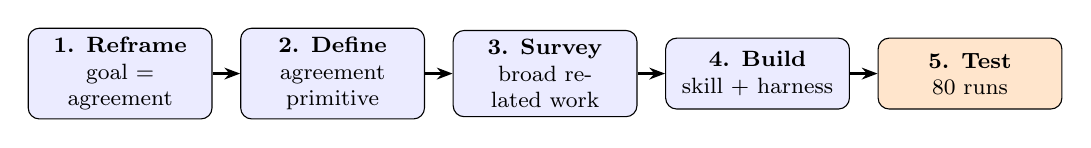
\begin{tikzpicture}[node distance=0.35cm]
    \node[box] (a) {\textbf{1. Reframe}\\goal = agreement};
    \node[box, right=of a] (b) {\textbf{2. Define}\\agreement primitive};
    \node[box, right=of b] (c) {\textbf{3. Survey}\\broad related work};
    \node[box, right=of c] (d) {\textbf{4. Build}\\skill + harness};
    \node[hl, right=of d] (e) {\textbf{5. Test}\\80 runs};
    \draw[arr] (a)--(b); \draw[arr] (b)--(c); \draw[arr] (c)--(d); \draw[arr] (d)--(e);
  \end{tikzpicture}

  \vspace{0.8em}
  \footnotesize
  \begin{tabular}{lll}
    \toprule
    Item & Output & Status \\
    \midrule
    Problem and use cases & 5 use cases, characterization axes & draft \\
    Definition & interface + 5 properties & draft \\
    Related work & 5 areas, positioning & done \\
    Prototype & \texttt{SKILL.md}, \texttt{agree.py}, 3 harness hooks & working \\
    Experiment & coding task, 8 conditions $\times$ 10 runs & pilot done \\
    \bottomrule
  \end{tabular}
\end{frame}

% ---------------------------------------------------------------
\subsection{Introduction}

\begin{frame}{Background and Motivation}
  \begin{columns}[T]
    \begin{column}{0.52\textwidth}
      \footnotesize\textbf{Background}: agents with different roles must make the same \textbf{shared choice} $\tau$; each option is valid, but mixing options breaks the result.\\[4pt]
      \begin{tabular}{ll}
        \toprule
        Use case & Shared choice $\tau$ \\
        \midrule
        Software & interface (types, error signal) \\
        Data analysis & outlier rule \\
        Scheduling & meeting slot \\
        Writing & terms, figures \\
        Operations & image version \\
        \bottomrule
      \end{tabular}
    \end{column}
    \begin{column}{0.46\textwidth}
      \footnotesize\textbf{Motivation}
      \begin{itemize}
        \item Two coding agents: $\sim$25\% success, about half of one agent; top failures are work overlap (33\%) and divergent architecture (30\%) [1]
        \item Agents break commitments even when they talk [1]
        \item Constraints dropped after context compaction: violations 0/100 $\to$ 30/100 [2]
      \end{itemize}
      \vspace{0.2em}
      $\Rightarrow$ agreeing once is not enough; outputs must \textbf{stay} consistent
    \end{column}
  \end{columns}
  \papercite{[1] A. Khatua, H. Zhu, P. Tran, et al. CooperBench: Why Coding Agents Cannot be Your Teammates Yet. \textit{COLM}, 2026. \;
  [2] Z. Wang, Y. Zhang, D. Lee, N. Baracaldo, Y. Yang. Lost in Context Compaction: When LLM Systems Drop Side Constraints. arXiv:2608.11242, 2026 (preprint).}
\end{frame}

\begin{frame}{Related Work: Five Areas}
  \footnotesize
  \begin{tabularx}{\textwidth}{l X X}
    \toprule
    Area & What it gives us & What is missing for us \\
    \midrule
    Distributed consensus \& commit [3,4,5] & agreement, validity, termination; commit/abort & assumes deterministic replicas \\
    Norms \& commitments in MAS [6,7] & monitoring compliance; regimentation vs.\ enforcement & norms written by designers, not LLMs \\
    LLM agreement / consensus [8,9] & LLMs agreeing on a value or answer & agreement ends at the answer \\
    LLM contracts \& coordination [10,11,12] & contracts, merge, runtime control & one enforcement point each \\
    Skills \& harness [13,14] & skills help; harness enforces rules & no skill vs.\ harness comparison \\
    \bottomrule
  \end{tabularx}
  \papercite{[3] L. Lamport, R. Shostak, M. Pease. The Byzantine Generals Problem. \textit{ACM TOPLAS}, 1982. \;
  [4] P. A. Bernstein, V. Hadzilacos, N. Goodman. \textit{Concurrency Control and Recovery in Database Systems}. 1987. \;
  [5] F. B. Schneider. Implementing Fault-Tolerant Services Using the State Machine Approach. \textit{ACM CSUR}, 1990. \;
  [6] M. P. Singh. An Ontology for Commitments in Multiagent Systems. \textit{AI and Law}, 1999. \;
  [7] D. Grossi, H. Aldewereld, F. Dignum. Ubi Lex, Ibi Poena: Designing Norm Enforcement in E-Institutions. \textit{COIN}, LNCS, 2007. \;
  [8] F. Berdoz, L. Rugli, R. Wattenhofer. Can AI Agents Agree? arXiv:2603.01213, 2026. \;
  [9] C. Ruan, Y. Wang, Z. Shi, J. Li. Reaching Agreement Among Reasoning LLM Agents. arXiv:2512.20184, 2025. \;
  [10] T. Wyse, K. Bustos, Y. Volkova, M. Kleiman-Weiner. Commitment To Cooperation With Self-Negotiated Contracts. arXiv:2607.22750, 2026. \;
  [11] J. Geng, G. Neubig. Effective Strategies for Asynchronous Software Engineering Agents. arXiv:2603.21489, 2026. \;
  [12] H. Lyu, D. Zhang, M. Wu, X. Wei, H. Chen. CoAgent: Concurrency Control for Multi-Agent Systems. arXiv:2606.15376, 2026. \;
  [13] X. Li, Y. Liu, W. Chen, et al. SkillsBench. arXiv:2602.12670, 2026. \;
  [14] Z. Xiang, L. Zheng, Y. Li, et al. GuardAgent. \textit{ICML}, 2025.}
\end{frame}

\begin{frame}{Positioning}
  \footnotesize
  \centering
  \begin{tabularx}{\textwidth}{l X X}
    \toprule
    When $\backslash$ Where & Agent (instructions / skill) & Harness (enforced) \\
    \midrule
    Before work & \textbf{this work (skill)} & Self-Negotiated Contracts [10]; \textbf{this work (gate)} \\
    On change & --- & CoAgent [12] \\
    At integration & --- & CAID [11]; \textbf{this work (end check)} \\
    Any time & CooperBench messaging [1] & --- \\
    \bottomrule
  \end{tabularx}

  \vspace{0.8em}
  \begin{tabular}{lll}
    \toprule
    & Closest work [10] & This work \\
    \midrule
    Why agents deviate & incentive (defect for gain) & honest drift (forget, mismatch) \\
    What is checked & actions & content of outputs \\
    Enforcement & always by environment & skill vs.\ harness, compared \\
    \bottomrule
  \end{tabular}
  \papercite{[1] Khatua et al., COLM 2026. \; [10] Wyse et al., arXiv:2607.22750, 2026. \; [11] Geng \& Neubig, arXiv:2603.21489, 2026. \; [12] Lyu et al., arXiv:2606.15376, 2026.}
\end{frame}

% ---------------------------------------------------------------
\subsection{Methods}
\begin{frame}{Model and Base Methods}
  \scriptsize
  \begin{columns}[T]
    \begin{column}{0.5\textwidth}
      \textbf{Model}\\[2pt]
      \begin{tabularx}{\linewidth}{l X}
        \toprule
        Agents & $a_1,\dots,a_n$, different roles, own workspace only \\
        Topic $\tau$ & shared choice; valid but incompatible options $D_\tau$ \\
        Decision $d$ & value from $D_\tau$, committed in shared log $L$ \\
        Output $o$ & what each agent produces after $d$ \\
        Conformance & $\mathrm{Conf}(o,d)$: does $o$ follow $d$? \\
        Failures & crash, context loss ($\approx$ crash-recovery), \textbf{silent divergence} \\
        Assumption & $L$ is reliable (single trusted store) \\
        \bottomrule
      \end{tabularx}
    \end{column}
    \begin{column}{0.48\textwidth}
      \textbf{Base methods (existing)}\\[2pt]
      \begin{tabularx}{\linewidth}{X l}
        \toprule
        What we take & Src \\
        \midrule
        Validity, Agreement, Termination & [3] \\
        Atomic commit: all accept $\Rightarrow$ commit, any veto $\Rightarrow$ abort & [4] \\
        SMR: same decisions + determinism $\Rightarrow$ same outputs & [5] \\
        Agent Skills: \texttt{SKILL.md} + scripts & [15] \\
        Claude Code hooks: block before tool / stop & [16] \\
        Two-role task, merged and tested & [1] \\
        \bottomrule
      \end{tabularx}\\[4pt]
      \textbf{New}: Conformance, since LLM agents are not deterministic
    \end{column}
  \end{columns}
  \papercite{[1] Khatua et al., COLM 2026. \; [3] Lamport et al., TOPLAS 1982. \; [4] Bernstein et al., 1987. \; [5] Schneider, ACM CSUR 1990. \;
  [15] Agent Skills specification, https://agentskills.io/specification. \; [16] Claude Code docs: Hooks, https://code.claude.com/docs/en/hooks (both accessed Oct 2026).}
\end{frame}


\begin{frame}{Proposed Method: Overview and Interface}
  \centering
  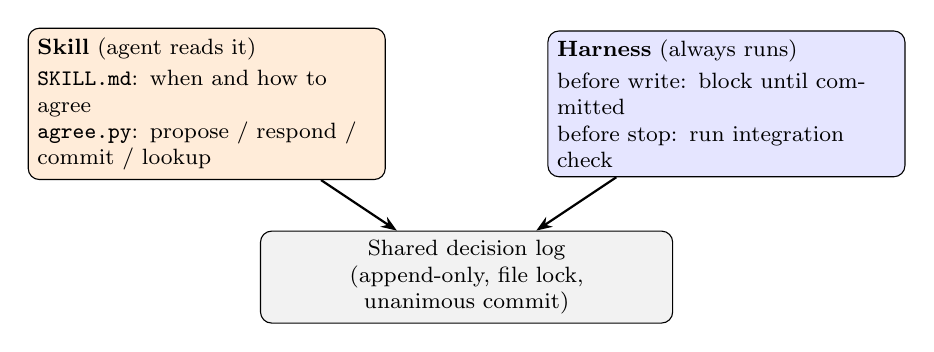
\begin{tikzpicture}[every node/.style={font=\footnotesize}]
    \node[draw, rounded corners, fill=orange!15, text width=4.3cm, align=left] (s) at (-3.3,0.8)
      {\textbf{Skill} (agent reads it)\\[2pt]\texttt{SKILL.md}: when and how to agree\\\texttt{agree.py}: propose / respond / commit / lookup};
    \node[draw, rounded corners, fill=blue!10, text width=4.3cm, align=left] (h) at (3.3,0.8)
      {\textbf{Harness} (always runs)\\[2pt]before write: block until committed\\before stop: run integration check};
    \node[draw, rounded corners, fill=gray!10, text width=5cm, align=center] (l) at (0,-1.4)
      {Shared decision log\\(append-only, file lock, unanimous commit)};
    \draw[arr] (s)--(l); \draw[arr] (h)--(l);
  \end{tikzpicture}

  \vspace{0.3em}
  \scriptsize
  \begin{tabular}{ll}
    \toprule
    Operation & Meaning \\
    \midrule
    \texttt{propose(}$\tau, d$\texttt{)} / \texttt{respond(}$r$\texttt{)} & open a version; $r\in\{$accept, object$\}$, one object aborts \\
    \texttt{commit(}$\tau$\texttt{)} / \texttt{lookup(}$\tau$\texttt{)} & all accepted $\Rightarrow$ append $d$ / read latest $d$ \\
    \texttt{check(}$o,\tau$\texttt{)} / \texttt{deviate(}$\tau$\texttt{)} & run $\mathrm{Conf}(o,d)$ / announce instead of diverging silently \\
    \bottomrule
  \end{tabular}
\end{frame}


\begin{frame}{Proposed Method: Detail (Harness Variants and Conditions)}
  \scriptsize
  \begin{columns}[T]
    \begin{column}{0.46\textwidth}
      \textbf{Harness variants}\\[2pt]
      \begin{tabularx}{\linewidth}{l X}
        \toprule
        Variant & Behavior \\
        \midrule
        Pre-write gate & cannot write own file until \texttt{interface} is committed \\
        End check & cannot stop if the merged code fails the example \\
        End + barrier & cannot stop until both are ready on the same file versions and the check passes \\
        \bottomrule
      \end{tabularx}
    \end{column}
    \begin{column}{0.5\textwidth}
      \textbf{Conditions} (10 runs each)\\[2pt]
      \begin{tabular}{lll}
        \toprule
        Condition & Where & When \\
        \midrule
        None & --- & --- \\
        Tool only (no procedure) & agent & any \\
        Inline procedure (prompt) & agent & before \\
        Skill (\texttt{SKILL.md}) & agent & before \\
        Pre-write gate & harness & before \\
        End check & harness & integration \\
        End check + barrier & harness & integration \\
        Skill + end check & both & both \\
        \bottomrule
      \end{tabular}
    \end{column}
  \end{columns}
\end{frame}

\begin{frame}{Experiment Task and Environment}
  \scriptsize
  \begin{columns}[T]
    \begin{column}{0.44\textwidth}
      \textbf{Task}: Agent 1 writes \texttt{pricing.py}; Agent 2 writes \texttt{invoice.py} using it. Separate folders, message board only. Merged and graded by 7 hidden tests. Agents are not told what must be decided.\\[4pt]
      \begin{tabular}{ll}
        \toprule
        Hidden shared choice & Options \\
        \midrule
        Price unit & cents / dollars / Decimal \\
        Unknown item & \texttt{None} / \texttt{KeyError} \\
        Discount & 10 / 0.1 / ``10\%'' \\
        \bottomrule
      \end{tabular}
    \end{column}
    \begin{column}{0.54\textwidth}
      \textbf{Environment}\\[2pt]
      \begin{tabular}{ll}
        \toprule
        CPU & Intel Xeon @ 2.80 GHz, 2 vCPUs \\
        GPU & none (models via Anthropic API) \\
        Memory & 7.8 GiB \\
        OS & Ubuntu 24.04.5 LTS (cloud container) \\
        Agent & Claude Code 2.1.312, headless (\texttt{claude -p}) \\
        Model & \texttt{claude-haiku-5-5}, max 40 turns \\
        Language & Python 3.13.16 \\
        Tools & Read, Write, Edit, Glob, Grep, limited Bash, Skill \\
        Runs & 8 conditions $\times$ 10, 5 trials in parallel \\
        \bottomrule
      \end{tabular}
    \end{column}
  \end{columns}
\end{frame}


% ---------------------------------------------------------------
\subsection{Results}
\begin{frame}{Results: Coordination Failures}
  \begin{columns}[c]
    \begin{column}{0.6\textwidth}
      \centering
      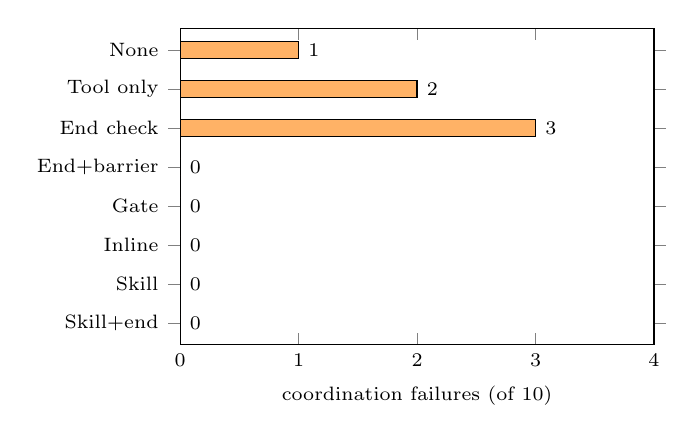
\begin{tikzpicture}
        \begin{axis}[xbar, width=7.6cm, height=5.6cm, xmin=0, xmax=4, bar width=6pt,
            symbolic y coords={Skill+end,Skill,Inline,Gate,End+barrier,End check,Tool only,None},
            ytick=data, yticklabel style={font=\scriptsize}, xticklabel style={font=\scriptsize},
            xlabel={coordination failures (of 10)}, label style={font=\scriptsize},
            nodes near coords, nodes near coords style={font=\scriptsize}, enlarge y limits=0.08]
          \addplot[fill=orange!60] coordinates {(0,Skill+end) (0,Skill) (0,Inline) (0,Gate) (0,End+barrier) (3,End check) (2,Tool only) (1,None)};
        \end{axis}
      \end{tikzpicture}
    \end{column}
    \begin{column}{0.38\textwidth}
      \footnotesize
      \begin{tabular}{lc}
        \toprule
        Condition & Success \\
        \midrule
        None & 8/10 \\
        Tool only & 8/10 \\
        Inline & 10/10 \\
        Skill & 8/10$^{*}$ \\
        Gate & 8/10$^{\dagger}$ \\
        End check & 7/10 \\
        End + barrier & 10/10 \\
        Skill + end & 10/10 \\
        \bottomrule
      \end{tabular}\\[3pt]
      {\tiny $^{*}$ both: own formatting bug\\ $^{\dagger}$ 1 formatting bug, 1 permission issue}
    \end{column}
  \end{columns}
  \vspace{0.3em}
  \footnotesize Procedure present 0/30 vs.\ absent 6/30 coordination failures (Fisher, one-sided $p=0.012$; grouping chosen after the fact).
\end{frame}

\begin{frame}{Results: What the Failures Looked Like}
  \small
  \textbf{All 6 coordination failures: crossing proposals}
  \vspace{0.3em}

  \footnotesize
  \begin{tabular}{rll}
    \toprule
    Time & Agent & Action \\
    \midrule
    0 s & Agent 2 & proposes ``unknown item $\Rightarrow$ return \texttt{None}'' \\
    9 s & Agent 1 & (before reading it) ``done: unknown item $\Rightarrow$ raise \texttt{KeyError}'' \\
     & Agent 2 & adapts to \texttt{KeyError}, finishes \\
    15 s & Agent 1 & reads the old proposal, switches to \texttt{None} \\
    \bottomrule
  \end{tabular}

  \vspace{0.8em}
  \begin{columns}[T]
    \begin{column}{0.48\textwidth}
      \centering\footnotesize\textbf{Mean wall time (s)}\\[2pt]
      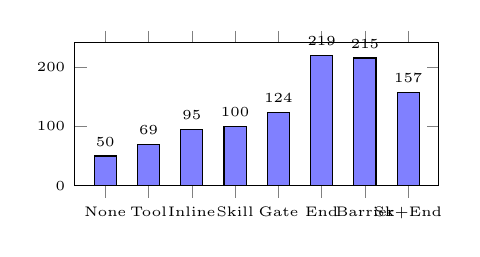
\begin{tikzpicture}
        \begin{axis}[ybar, width=6.2cm, height=3.4cm, ymin=0, bar width=8pt,
            symbolic x coords={None,Tool,Inline,Skill,Gate,End,Barrier,Sk+End}, xtick=data,
            ticklabel style={font=\tiny}, nodes near coords, nodes near coords style={font=\tiny}]
          \addplot[fill=blue!50] coordinates {(None,50) (Tool,69) (Inline,95) (Skill,100) (Gate,124) (End,219) (Barrier,215) (Sk+End,157)};
        \end{axis}
      \end{tikzpicture}
    \end{column}
    \begin{column}{0.5\textwidth}
      \footnotesize
      \begin{itemize}
        \item No single committed value $\Rightarrow$ concurrent updates swap
        \item With a procedure, one value is committed first
        \item End check found the mismatch, but the partner had already exited
      \end{itemize}
    \end{column}
  \end{columns}
\end{frame}

% ---------------------------------------------------------------
\subsection{Discussion}
\begin{frame}{Discussion}
  \small
  \textbf{What the pilot suggests}
  \begin{enumerate}
    \item The \textbf{procedure} matters, not the tool (tool only = no change)
    \item Skill format showed no extra effect over the same text in the prompt
    \item Harness \textbf{timing} matters: an end check needs a barrier (like two-phase commit)
    \item The cost is mostly time, not tokens
  \end{enumerate}
  \textbf{Why not Paxos or Raft?} One trusted log, no message loss, and with 2 agents a majority is everyone; failures came from no commit point, not crashes.

  \vspace{0.4em}
  \textbf{Limitations}
  \begin{itemize}
    \item 10 runs per condition, one model, one synthetic task; baseline already 8/10
    \item Two experimenter bugs found and fixed (gate blocked the agreement tool; permission patterns)
  \end{itemize}
\end{frame}

% ===============================================================
\section{Questions and Next Week}
\begin{frame}{Question List and Next Week}
  \footnotesize
  \textbf{Questions}
  \begin{enumerate}
    \item \textbf{Novelty}: normative MAS already monitors compliance. Is ``agents negotiate $d$ themselves + output conformance'' enough?
    \item \textbf{Commit rule}: unanimous, owner decides, or majority? Default or variable?
    \item \textbf{Skill vs.\ inline}: if the format adds nothing, should the axis be ``procedure vs.\ enforcement''?
    \item \textbf{Task realism}: is a synthetic task acceptable, or must I use an existing benchmark (e.g., CooperBench)?
    \item \textbf{Log model}: is a single trusted log acceptable, or should the log be replicated?
  \end{enumerate}
  \textbf{Next week}
  \begin{itemize}
    \item Confirmatory run (pre-registered): none / inline / skill, 30 runs each
    \item Harder task: longer work, mid-task spec change, 3 agents
    \item Second use case with the same skill; fix permission patterns
  \end{itemize}
\end{frame}

% ===============================================================

% ===============================================================
\begin{frame}{References}
  \tiny
  \begin{multicols}{2}
  \begin{thebibliography}{16}
    \bibitem{cooper} A. Khatua, H. Zhu, P. Tran, et al. CooperBench: Why Coding Agents Cannot be Your Teammates Yet. \textit{COLM}, 2026.
    \bibitem{lcc} Z. Wang, Y. Zhang, D. Lee, N. Baracaldo, Y. Yang. Lost in Context Compaction: When LLM Systems Drop Side Constraints. arXiv:2608.11242, 2026.
    \bibitem{lsp} L. Lamport, R. Shostak, M. Pease. The Byzantine Generals Problem. \textit{ACM TOPLAS} 4(3):382--401, 1982.
    \bibitem{bhg} P. A. Bernstein, V. Hadzilacos, N. Goodman. \textit{Concurrency Control and Recovery in Database Systems}. Addison-Wesley, 1987.
    \bibitem{smr} F. B. Schneider. Implementing Fault-Tolerant Services Using the State Machine Approach: A Tutorial. \textit{ACM Computing Surveys} 22(4):299--319, 1990.
    \bibitem{singh} M. P. Singh. An Ontology for Commitments in Multiagent Systems: Toward a Unification of Normative Concepts. \textit{Artificial Intelligence and Law} 7:97--113, 1999.
    \bibitem{grossi} D. Grossi, H. Aldewereld, F. Dignum. Ubi Lex, Ibi Poena: Designing Norm Enforcement in E-Institutions. \textit{COIN}, LNCS, 2007.
    \bibitem{agree} F. Berdoz, L. Rugli, R. Wattenhofer. Can AI Agents Agree? arXiv:2603.01213, 2026.
    \bibitem{aegean} C. Ruan, Y. Wang, Z. Shi, J. Li. Reaching Agreement Among Reasoning LLM Agents. arXiv:2512.20184, 2025.
    \bibitem{snc} T. Wyse, K. Bustos, Y. Volkova, M. Kleiman-Weiner. Commitment To Cooperation With Self-Negotiated Contracts. arXiv:2607.22750, 2026.
    \bibitem{caid} J. Geng, G. Neubig. Effective Strategies for Asynchronous Software Engineering Agents. arXiv:2603.21489, 2026.
    \bibitem{coagent} H. Lyu, D. Zhang, M. Wu, X. Wei, H. Chen. CoAgent: Concurrency Control for Multi-Agent Systems. arXiv:2606.15376, 2026.
    \bibitem{skillsbench} X. Li, Y. Liu, W. Chen, et al. SkillsBench: Benchmarking How Well Agent Skills Work Across Diverse Tasks. arXiv:2602.12670, 2026.
    \bibitem{guard} Z. Xiang, L. Zheng, Y. Li, et al. GuardAgent: Safeguard LLM Agents by a Guard Agent via Knowledge-Enabled Reasoning. \textit{ICML}, 2025.
    \bibitem{skills} Agent Skills specification. https://agentskills.io/specification (accessed Oct 2026).
    \bibitem{hooks} Claude Code documentation: Hooks. https://code.claude.com/docs/en/hooks (accessed Oct 2026).
  \end{thebibliography}
  \end{multicols}
\end{frame}

\end{document}
